\documentclass{article}

\def\npart {II}
\def\nyear {2017}
\def\nterm {Lent}
\def\nlecturer{Dr R.\ Camina}
\def\ncourse{Coding and Cryptography}
\ifx \nauthor\undefined
  \def\nauthor{Bhavik Mehta}
\else
\fi

\author{Based on lectures by \nlecturer \\\small Notes taken by \nauthor}
\date{\nterm\ \nyear}
\title{Part \npart\ -- \ncourse}

\usepackage[utf8]{inputenc}
\usepackage{amsmath}
\usepackage{amsthm}
\usepackage{amssymb}
\usepackage{enumerate}
\usepackage{mathtools}
\usepackage{graphicx}
\usepackage[dvipsnames]{xcolor}
\usepackage{tikz}
\usepackage{wrapfig}
\usepackage{centernot}
\usepackage{float}
\usepackage{braket}
\usepackage[hypcap=true]{caption}
\usepackage{enumitem}
\usepackage[colorlinks=true, linkcolor=mblue]{hyperref}
\usepackage[nameinlink,noabbrev]{cleveref}
\usepackage{nameref}
\usepackage[margin=1.5in]{geometry}

% Theorems
\theoremstyle{definition}
\newtheorem*{aim}{Aim}
\newtheorem*{axiom}{Axiom}
\newtheorem*{claim}{Claim}
\newtheorem*{cor}{Corollary}
\newtheorem*{conjecture}{Conjecture}
\newtheorem*{defi}{Definition}
\newtheorem*{eg}{Example}
\newtheorem*{ex}{Exercise}
\newtheorem*{fact}{Fact}
\newtheorem*{law}{Law}
\newtheorem*{lemma}{Lemma}
\newtheorem*{notation}{Notation}
\newtheorem*{prop}{Proposition}
\newtheorem*{question}{Question}
\newtheorem*{rrule}{Rule}
\newtheorem*{thm}{Theorem}
\newtheorem*{assumption}{Assumption}

\newtheorem*{remark}{Remark}
\newtheorem*{warning}{Warning}
\newtheorem*{exercise}{Exercise}

% \newcommand{\nthmautorefname}{Theorem}

\newtheorem{nthm}{Theorem}[section]
\newtheorem{nlemma}[nthm]{Lemma}
\newtheorem{nprop}[nthm]{Proposition}
\newtheorem{ncor}[nthm]{Corollary}
\newtheorem{ndef}[nthm]{Definition}

% Special sets
\newcommand{\C}{\mathbb{C}}
\newcommand{\N}{\mathbb{N}}
\newcommand{\Q}{\mathbb{Q}}
\newcommand{\R}{\mathbb{R}}
\newcommand{\Z}{\mathbb{Z}}

\newcommand{\abs}[1]{\left\lvert #1\right\rvert}
\newcommand{\norm}[1]{\left\lVert #1\right\rVert}
\renewcommand{\vec}[1]{\boldsymbol{\mathbf{#1}}}

\let\Im\relax
\let\Re\relax

\DeclareMathOperator{\Im}{Im}
\DeclareMathOperator{\Re}{Re}
\DeclareMathOperator{\id}{id}

\definecolor{mblue}{rgb}{0., 0.05, 0.6}


% preamble
\usepackage{tikz}
\usetikzlibrary{arrows,decorations.pathmorphing,decorations.markings,positioning}
\renewcommand{\thesection}{\Roman{section}}
% and here we go!

\begin{document}
\maketitle
\tableofcontents

\section*{Introduction to communication channels and coding}
For example, given a message $m$=`Call me!' which we wish to send by email, first encode as binary strings using ASCII.
So, $f(C) = 1000011, f(a) = 1100001$, and $f^*(m) = 1000011\ 1100001 \dots 0100001$.
% picture
\tikzstyle{block} = [rectangle, draw, fill=YellowOrange!20,
    text width=4em,
    text centered,
    minimum height=2em
    ]
\begin{center}
    \begin{tikzpicture}[node distance=3cm]
        \node (s) at (0, 0) [block] {source};
        % this is kind of horrible but it works :/
        \node (e) at (3, 0) [block] {encoder};
        \node (d) at (8, 0) [block] {decoder};
        \node (r) at (11, 0) [block] {receiver};
        \draw [->, shorten > =0.1em, thick] (s) -- (e);
        \draw [->, shorten > =0.1em, thick, decorate, decoration={amplitude=1.5mm,
            segment length=10mm,
            snake, post length=1mm}] (e) -- (d)
            node [above=0.5em,align=center,midway] {channel}
            node [below=0.5em,align=center,midway,color=red] {errors};

        \draw [->, shorten > =0.1em, thick] (d) -- (r);
    \end{tikzpicture}
\end{center}

\textbf{Basic problem:} Given a source and a channel (described probabilistically) we aim to design an encoder and a decoder in order to transmit information both economically and reliably (coding) and maybe also to preserve privacy (cryptography).

\begin{eg}
\leavevmode
\begin{itemize}
    \item `economically'
    Morse code: common letters have shorter codewords:
    % A .-, E ., Q --.--
    \item `reliably'
    Every book has an ISBN of form $a_1 a_2 \dotsc a_{10}$ where $a_i \in \{0, 1, \dotsc, 9\}$ for $1 \leq i \leq 9$, $a_{10} \in \{0, 1, \dotsc, 9, X\}$ such that
    \begin{equation*}
        10 a_1 + 9 a_2 + \dotsc + a_{10} \equiv 0 \pmod{11}
    \end{equation*}
    so errors can be detected (but not corrected).
    Similarly a 13-digit ISBN has
    \begin{equation*}
        x_1 + 3 x_2 + x_3 + 3 x_4 + \dotsc + 3 x_{12} + x_{13} \equiv 0 \pmod{10}
    \end{equation*}
    for $0 \leq x_i \leq 10$, doesn't necessarily spot transpositions.
\item `preserve privacy' e.g. RSA.
\end{itemize}
\end{eg}

A \textbf{communication channel} takes letters from an input alphabet $\Sigma_1 = \{a_1, \dotsc, a_r\}$ and emits letters form an output alphabet $\Sigma_2 = \{b_1, \dotsc, b_s\}$.

A channel is determined by the probabilities
\begin{equation*}
    P(y_1 \dotsc y_k \text{ received} \mid x_1 \dotsc x_k \text{ sent})
\end{equation*}

\begin{defi}[Discrete memoryless channel]\hypertarget{def:dmc}
    A \textbf{discrete memoryless channel} (DMC) is a channel for which
    \begin{equation*}
        P_{ij} = P(b_j \text{ received} \mid a_i \text{ sent})
    \end{equation*}
    is the same each time the channel is used and is independent of all past and future uses.
\end{defi}

The channel matrix is the $r \times s$ matrix with entries $p_{ij}$ (note the rows sum to 1).

\begin{eg}
    Binary Symmetric Channel (BSC) has $\Sigma_1 = \Sigma_2 = \{0, 1\}$, $0 \leq p \leq 1$:
    \begin{center}
        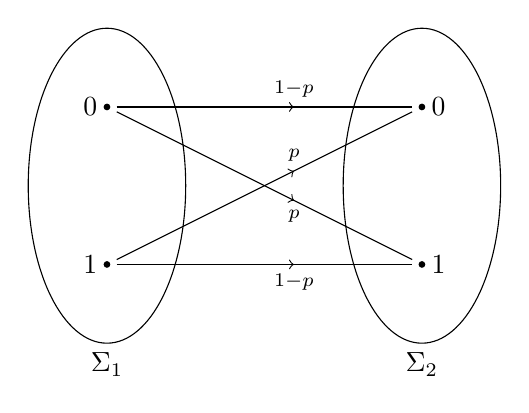
\begin{tikzpicture}
            \draw (-2, 0) circle [x radius=1cm, y radius=2cm] node [below=2cm] {$\Sigma_1$};
            \draw ( 2, 0) circle [x radius=1cm, y radius=2cm] node [below=2cm] {$\Sigma_2$};

            \node (0l) at (-2, 1) {};
            \node (1l) at (-2,-1) {};

            \node (0r) at (2, 1) {};
            \node (1r) at (2,-1) {};

            \filldraw (0l) circle (1pt) node [left] {0};
            \filldraw (1l) circle (1pt) node [left] {1};
            \filldraw (0r) circle (1pt) node [right] {0};
            \filldraw (1r) circle (1pt) node [right] {1};

            \begin{scope}[decoration={
                markings,
                mark=at position 0.6 with {\arrow{>}}}
                ]
                \draw[postaction={decorate}] (0l) -- (0r)
                    node [above,align=center,pos=0.6] {$\scriptstyle 1-p$};
                \draw[postaction={decorate}] (0l) -- (1r)
                    node [below,align=center,pos=0.6] {$\scriptstyle p$};
                \draw[postaction={decorate}] (1l) -- (0r)
                    node [above,align=center,pos=0.6] {$\scriptstyle p$};
                \draw[postaction={decorate}] (1l) -- (1r)
                    node [below,align=center,pos=0.6] {$\scriptstyle 1-p$};
            \end{scope}
        \end{tikzpicture}
    \end{center}
    with channel matrix
    \begin{equation*}
        \begin{pmatrix}
            1-p & p \\ p & 1-p
        \end{pmatrix}
    \end{equation*}
    i.e. $p$ is the probability a symbol is mistransmitted.


    Another example is given by the Binary Erasure channel, $\Sigma_1 \{0, 1\}$, $\Sigma_2 = \{0, 1, *\}$ and $0 \leq p \leq 1$.
    \begin{center}
        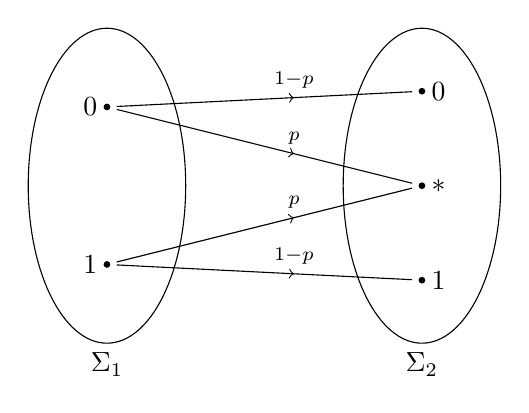
\begin{tikzpicture}
            \draw (-2, 0) circle [x radius=1cm, y radius=2cm] node [below=2cm] {$\Sigma_1$};
            \draw ( 2, 0) circle [x radius=1cm, y radius=2cm] node [below=2cm] {$\Sigma_2$};

            \node (0l) at (-2, 1) {};
            \node (1l) at (-2,-1) {};

            \node (0r) at (2, 1.2) {};
            \node (*r) at (2,   0) {};
            \node (1r) at (2,-1.2) {};

            \filldraw (0l) circle (1pt) node [left] {0};
            \filldraw (1l) circle (1pt) node [left] {1};
            \filldraw (0r) circle (1pt) node [right] {0};
            \filldraw (*r) circle (1pt) node [right] {$*$};
            \filldraw (1r) circle (1pt) node [right] {1};

            \begin{scope}[decoration={
                markings,
                mark=at position 0.6 with {\arrow{>}}}
                ]
                \draw[postaction={decorate}] (0l) -- (0r)
                    node [above,align=center,pos=0.6] {$\scriptstyle 1-p$};
                \draw[postaction={decorate}] (0l) -- (*r)
                    node [above,align=center,pos=0.6] {$\scriptstyle p$};
                \draw[postaction={decorate}] (1l) -- (*r)
                    node [above,align=center,pos=0.6] {$\scriptstyle p$};
                \draw[postaction={decorate}] (1l) -- (1r)
                    node [above,align=center,pos=0.6] {$\scriptstyle 1-p$};
            \end{scope}
        \end{tikzpicture}
    \end{center}
    with channel matrix
    \begin{equation*}
        \begin{pmatrix}
            1-p & p & 0 \\
            0 & p & 1-p
        \end{pmatrix}
    \end{equation*}
    i.e. $p$ is the probability a symbol can't be read.
\end{eg}

Informally, a channel's capacity is the highest rate at which information can be reliably transmitted over the channel.
Rate refers to units of information per unit time, which we want to be high. Similarly, reliably means we want an arbitrarily small error probability.

\clearpage
\section{Noiseless Coding}
\begin{notation}
    For $\Sigma$ an alphabet, let $\Sigma^* = \bigcup_{n \geq 0} \Sigma^n$ be the set of all finite strings of elements of $\Sigma$.
\end{notation}
If $x = x_1 \dotsc x_r$, $y = y_1 \dotsc y_s$ are strings from $\Sigma$, write $xy$ for the concatenation $x_1 \dotsc x_r y_1 \dotsc y_s$.
Further, $\abs{x_1 \dotsc x_r y_1 \dotsc y_s} = r+s$, length of string.
\begin{defi}[Code]\hypertarget{def:code}
    Let $\Sigma_1, \Sigma_2$ be two alphabets. A \textbf{code} is a function $f: \Sigma_1 \to \Sigma_2^*$. The strings $f(x)$ for $x \in \Sigma_1$ are called \textbf{codewords}.
\end{defi}
\begin{eg}
    \leavevmode
    \begin{enumerate}[label=\arabic*)] % 1)
        \item
            Greek fire \hyperlink{def:code}{code}:
            \begin{align*}
                \Sigma_1 &= \{\alpha, \beta, \gamma, \dotsc, \omega\} \quad \text{ 24 letters} \\
                \Sigma_2 &= \{1, 2, 3, 4, 5\}
            \end{align*}
            so, $\alpha \mapsto 11, \beta \mapsto 12, \dotsc, \omega \mapsto 54$.
        \item
            $\Sigma_1 = $ \{all words in the dictionary\}, and $\Sigma_2 = $\{A, B, $\dotsc$, Z, \} % add space symbol
            and $f$=`spell the word and a space'.
    \end{enumerate}
\end{eg}
We send a message $x_1, \dotsc, x_n \in \Sigma_1^*$ as $f(x_1) f(x_2) \dotsm f(x_n) \in \Sigma_2^*$ i.e. extend $f$ to $f^* : \Sigma_1^* \to \Sigma_2^*$.

\begin{defi}[Decipherable]\hypertarget{def:decipherable}
    A \hyperlink{def:code}{code} $f$ is \textbf{decipherable} if $f^*$ is injective, i.e. every string from $\Sigma_2$ arises from at most one message.
    Clearly we need $f$ injective, but this is not enough.
\end{defi}
\end{document}
